% Copyright (c) 2010 Jérémie DECOCK

\documentclass{beamer}
\usepackage[utf8]{inputenc}
\usepackage[frenchb]{babel}
\usepackage{hyperref}
\usepackage{subfigure}
%\usepackage[pdftex]{graphicx}
%\usepackage{natbib}
\usepackage{listings}
%\usepackage{algorithmic}
\usepackage{calc}

\lstset{
    basicstyle=\small,                                % print whole listing small
    keywordstyle=\color{black}\bfseries\underbar,     % underlined bold black keywords
    identifierstyle=,                                 % nothing happens
    commentstyle=\color{white},                       % white comments
    stringstyle=\ttfamily,                            % typewriter type for strings
    showstringspaces=false                            % no special string spaces
}


\hypersetup{
	pdftoolbar=true,                                          % show Acrobat’s toolbar ?
	pdfmenubar=true,                                          % show Acrobat’s menu ?
	pdffitwindow=true,                                        % page fit to window when opened
	pdftitle={Neurosciences computationnelles et algorithmes évolutionnistes},                                % title
	pdfauthor={Jérémie DECOCK},                                                                               % author
	pdfsubject={Les algorithmes évolutionnistes utilisés dans le cadre des neurosciences computationnelles},  % subject of the document
	pdfnewwindow=true,                                                                                        % links in new window
	pdfkeywords={algorithmes évolutionnistes, neurosciences computationnelles},                               % list of keywords
	colorlinks=true,                                          % false: boxed links; true: colored links
	linkcolor=black,                                          % color of internal links
	citecolor=black,                                          % color of links to bibliography
	filecolor=black,                                          % color of file links
	urlcolor=black                                            % color of external links
}

%\usetheme{Singapore}

\title{Les algorithmes évolutionnistes utilisés dans le cadre des neurosciences computationnelles}
\author{Jérémie \bsc{Decock}}
\institute{UPMC}
\date{29 janvier 2010}

\begin{document}

\begin{frame}
\titlepage
\end{frame}

%%%%%%%%%%%%%%%%%%%%%%%%%%%%%%%%%%%%%%%

\begin{frame}
\frametitle{But des neurosciences computationnelles et des algorithmes évolutionnistes~?}
Algorithmes évolutionnistes
\begin{itemize}
	\item trouver des solutions satisfaisantes à des problèmes d'optimisation
\end{itemize}
~\\
Neurosciences computationnelles
\begin{itemize}
	\item découvrir les principes computationnels des fonctions cérébrales et de l'activité neuronale
\end{itemize}
\end{frame}

%%%%%%%%%%%%%%%%%%%%%%%%%%%%%%%%%%%%%%%

\begin{frame}
\frametitle{Plan}
%\tableofcontents
\tableofcontents[sectionstyle=show/show,subsectionstyle=hide/hide/hide]
\end{frame}

%%%%%%%%%%%%%%%%%%%%%%%%%%%%%%%%%%%%%%%

\section{Introduction aux algorithmes évolutionnistes}
\begin{frame}
\begin{center}
{\LARGE Introduction aux algorithmes évolutionnistes}
\end{center}
\end{frame}


\begin{frame}
\frametitle{Définition}
Les algorithmes évolutionnistes
\begin{itemize}
	\item algorithmes stochastiques itératifs
	\item résoudre des problèmes d'optimisation
\end{itemize}
\begin{center}
        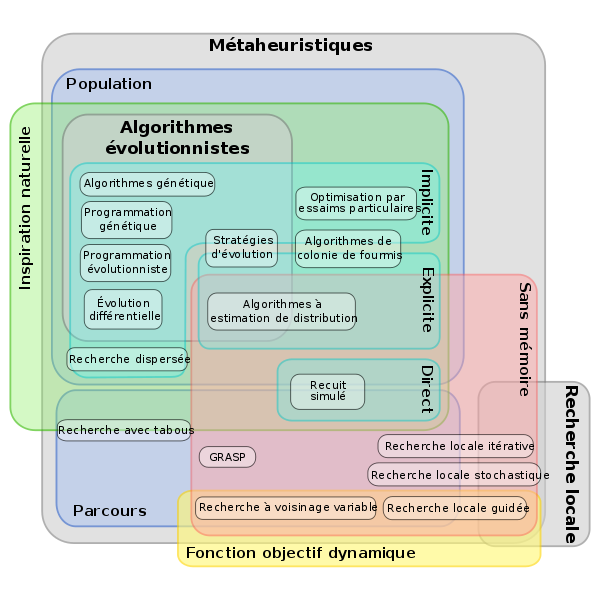
\includegraphics[width=.60\linewidth]{images/metaheuristiques}
\end{center}
\end{frame}


\begin{frame}
\frametitle{Principe}
S'inspire de la théorie synthétique de l'évolution (neodarwinisme)
\begin{itemize}
	\item les caractéristiques "innées" sont codées dans les gènes
	\item chaque individu a un génotype unique
	\item le phénotype de chacun est plus ou moins adapté à l'environnement
	\item les gènes des parents sont croisés pour former le génotype de leurs enfants lors de la reproduction
	\item des mutations peuvent avoir lieu aléatoirement sur le génome des nouveaux individus
	\item les individus dont le phénotype inadapté à leur environnement ont moins de chance de survivre jusqu'à la reproduction
\end{itemize}
\end{frame}

%\begin{frame}[containsverbatim]
\begin{frame}[fragile]
\frametitle{Fonctionnement}
Parallèle AE/Neodarwinisme
\begin{itemize}
	\item individu = une solution potentielle du problème à résoudre
	\item genome = le codage des solutions 
\end{itemize}
~\\
\begin{lstlisting}[frame=single]
begin Evolutionary computation
    t := 0
    P(t) := initialize_population() 
    evaluate(P(t))
    while not done do
        t := t+1
        P'(t) := select_parents(P(t))
        crossover(P'(t))
        mutate(P'(t))
        evaluate(P'(t))
        P(t+1) := select_survivals(P'(t),P(t))
    end while
end Evolutionary computation
\end{lstlisting}
\end{frame}



\begin{frame}
\frametitle{Fonctionnement}
\begin{center}
        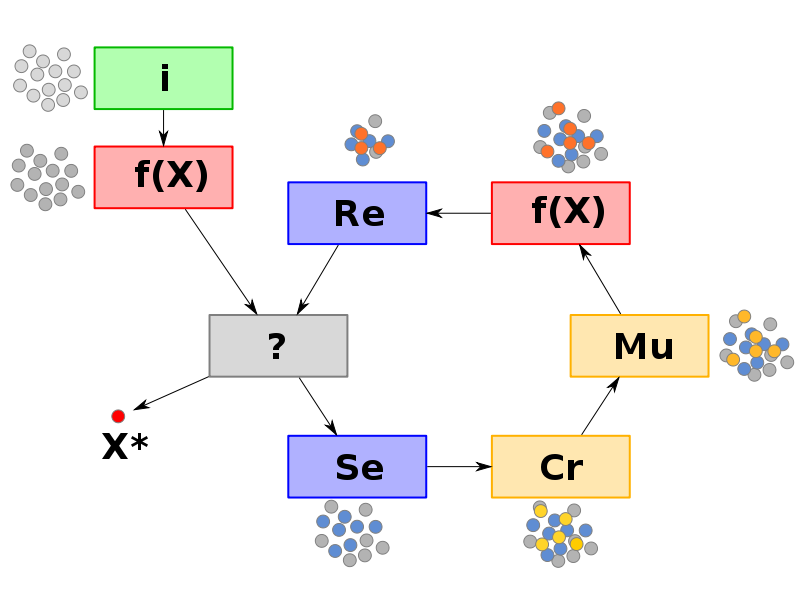
\includegraphics[width=.80\linewidth]{images/ae}
\end{center}
\end{frame}


\begin{frame}
\frametitle{Problèmes couverts}
Problèmes d'optimisation : recherche d'optimums globaux\\
~\\
Forces
\begin{itemize}
	\item évitent les optimums locaux                                                  % algorithme stochastique itératif
	\item facilement transposables sur de nombreux types de problèmes                 % (populaire)
	\item réussissent là où les méthodes déterministes échouent
    \begin{itemize}
        \item problèmes NP-complet
        \item problèmes avec une fonction objectif discontinue et/ou non dérivable
    \end{itemize}
\end{itemize}
~\\
Faiblesses
\begin{itemize}
	\item recherche d'optimums \og~satisfaisants~\fg                                 % metaheuristique
	\item pas de résultat optimal garanti en temps fini                             % metaheuristique
	%\item on peut trouver des résultats différents d'une optimisation à l'autre     % algo stochatique itératif => non déterministe (+ on ne sait rien sur leur proximité à l'optimum global)
	\item on peut trouver des résultats différents à chaque exécution               % algo stochatique itératif => non déterministe (+ on ne sait rien sur leur proximité à l'optimum global)
	\item généralement moins rapides que les méthodes déterministe
\end{itemize}
\end{frame}


\begin{frame}
\frametitle{Quels attraits pour les neurosciences computationnelles}
Modèles calculables des fonctions cérébrales et des processus cognitifs\\
~\\
Optimisation sur des modèles
\begin{itemize}
	\item dynamiques
	\item non dérivables
	\item non continus
    \item comportant de nombreux paramètres
\end{itemize}
~\\
Recherche d'un optimum global
\end{frame}

%%%%%%%%%%%%%%%%%%%%%%%%%%%%%%%%%%%%%%%

\section{L'utilisation des algorithmes évolutionnistes dans le contexte des neurosciences computationnelles}
\begin{frame}
\begin{center}
{\LARGE L'utilisation des algorithmes évolutionnistes dans le contexte des neurosciences computationnelles}
\end{center}
\end{frame}

\subsection{L'analyse et l'optimisation de modèles biologiques}

\begin{frame}{Plan - \secname}
    \tableofcontents[sectionstyle=hide/hide,subsectionstyle=show/shaded/hide ]
\end{frame}

%\begin{frame}
%\frametitle{L'utilisation des algorithmes évolutionnistes dans les neurosciences computationnelles}
%\begin{itemize}
%	\item l'analyse et l'optimisation de modèles biologiques
%    \item l'optimisation de modèles \og~boite noire~\fg
%    \item l'observation de l'activité cérébrale
%\end{itemize}
%\end{frame}

\begin{frame}
\frametitle{L'analyse et l'optimisation de modèles biologiques}
Le contexte
\begin{itemize}
    \item besoin de modèles simulant le comportement des structures nerveuses
    \item pour étudier leurs capacités computationnelles
    \item ces modèles sont de plus en plus complexes
    \item ils renferment de plus en plus de paramètres à optimiser
    \item pour obtenir un modèle fidèle à la réalité
\end{itemize}
~\\
Les algorithmes évolutionnistes permettent d'automatiser cette tâche
\end{frame}


\begin{frame}
\frametitle{L'analyse et l'optimisation de modèles biologiques}
Exemples d'utilisation
\begin{itemize}
    \item modélisation des propriétés computationnelles d'un neurone $[$KPK05$]$
    \item modélisation de la dynamique du traitement de l'information dans le neocortex $[$SIK04$]$
    \item modélisation et simulation des colonnes neocorticales (Blue Brain Project) $[$MAR06$]$ $[$DBG07$]$
\end{itemize}
\end{frame}


%\begin{frame}
%\frametitle{L'analyse et l'optimisation de modèles biologiques}
%\framesubtitle{Modélisation des propriétés computationnelles d'un neurone isolé}
%Description du modèle
%~\\
%Motivations
%\begin{itemize}
%	\item ...
%\end{itemize}
%~\\
%Expérience sans AE
%~\\
%Expérience avec AE
%\begin{itemize}
%	\item Indiv
%	\item Gène 
%	\item Fitness 
%\end{itemize}
%~\\
%Résultat
%\begin{itemize}
%	\item Est-ce que c'est justifié ?
%	\item Quels gains apportés ?
%\end{itemize}
%\end{frame}


%\begin{frame}
%\frametitle{L'analyse et l'optimisation de modèles biologiques}
%\framesubtitle{Modélisation de la dynamique du traitement de l'information dans le neocortex}
%Description du modèle
%~\\
%Motivations
%\begin{itemize}
%	\item ...
%\end{itemize}
%~\\
%Expérience sans AE
%~\\
%Expérience avec AE
%\begin{itemize}
%	\item Indiv
%	\item Gène 
%	\item Fitness 
%\end{itemize}
%~\\
%Résultat
%\begin{itemize}
%	\item Est-ce que c'est justifié ?
%	\item Quels gains apportés ?
%\end{itemize}
%\end{frame}


\subsection{L'optimisation de modèles \og~boite noire~\fg}

\begin{frame}{Plan - \secname}
    \tableofcontents[sectionstyle=hide/hide,subsectionstyle=show/shaded/hide ]
\end{frame}


\begin{frame}
\frametitle{L'optimisation de modèles \og~boite noire~\fg}
Le contexte
\begin{itemize}
    \item optimiser les performances d'un modèle
    \item sans chercher à comprendre ou interpréter les résultats (applications pratiques)
\end{itemize}
~\\
Les besoins
\begin{itemize}
    \item un outil capable de résoudre n'importe quel type de problème d'optimisation
    \item ayant recours à des fonctions objectif non dérivables et discontinues
    \item qui ne soit pas piégé par un optimum local
    \item dont l'implémentation doit être simple et générique
    \item évitant tout réglages qui impliquent une compréhension profonde du problème
\end{itemize}
\end{frame}


\begin{frame}
\frametitle{L'optimisation de modèles \og~boite noire~\fg}
Les algorithmes évolutionnistes répondent à ces attentes\\
~\\
Exemple d'utilisation %\og~boite noire~\fg : robotique bio-inspirée (behavior-based robotics) % sélection du comportement à manifester, face à l'état perçu du monde
\begin{itemize}
    \item behavior-based robotics
    \begin{itemize}
        \item optimisation de modèles des ganglions de la base $[$WLCH07$]$
        \item optimisation d'un modèle des formations réticulées $[$HGP05$]$
    \end{itemize}
\end{itemize}
%~\\
%Structure biologique
%\begin{itemize}
%%	\item centre de contrôle du cerveau présente une architecture en couches
%	\item De nombreuses structures (couches basses) génèrent des actions à destination du système nerveux périphérique
%	\item Ces actions sont parfois contradictoires et doivent être filtrées par un médiateur (couche haute)
%	\item Deux structures supposées remplir ce rôle de médiateur ont été identifiées par les neuroscientifiques
%	\item les ganglions de la base et les formations réticulées
%\end{itemize}
\end{frame}


%\begin{frame}
%\frametitle{L'optimisation de modèles \og~boite noire~\fg}
%\framesubtitle{Modélisation des ganglions de la base}
%Description du modèle
%~\\
%Motivations
%\begin{itemize}
%	\item ...
%\end{itemize}
%~\\
%Expérience sans AE
%~\\
%Expérience avec AE
%\begin{itemize}
%	\item Indiv
%	\item Gène 
%	\item Fitness 
%\end{itemize}
%~\\
%Résultat
%\begin{itemize}
%	\item Est-ce que c'est justifié ?
%	\item Quels gains apportés ?
%\end{itemize}
%\end{frame}
%
%
%\begin{frame}
%\frametitle{L'optimisation de modèles \og~boite noire~\fg}
%\framesubtitle{Modélisation des formations réticulées}
%Description du modèle
%~\\
%Motivations
%\begin{itemize}
%	\item ...
%\end{itemize}
%~\\
%Expérience sans AE
%~\\
%Expérience avec AE
%\begin{itemize}
%	\item Indiv
%	\item Gène 
%	\item Fitness 
%\end{itemize}
%~\\
%Résultat
%\begin{itemize}
%	\item Est-ce que c'est justifié~?
%	\item Quels gains apportés~?
%\end{itemize}
%\end{frame}


\subsection{L'observation de l'activité cérébrale}

\begin{frame}{Plan - \secname}
    \tableofcontents[sectionstyle=hide/hide,subsectionstyle=show/shaded/hide ]
\end{frame}


\begin{frame}
\frametitle{L'observation de l'activité cérébrale}
Exemple : l'électro-encéphalographie (EEG)
\begin{itemize}
	\item mesure de l'activité électrique du cerveau
	\item renseigne sur l'activité cérébrale du cortex
	\item précis dans le temps mais pas dans l'espace           % signal diffu et bruité
\end{itemize}
~\\
%\begin{center}
%        \includegraphics[width=.40\linewidth]{images/eeg1}
%\end{center}

%\begin{figure}
%   \includegraphics[]{eeg1}
%\end{figure}

\begin{figure}
    \centering
    \subfigure{\includegraphics[width=.40\linewidth,height=.30\linewidth]{images/eeg1}}~~~
    \subfigure{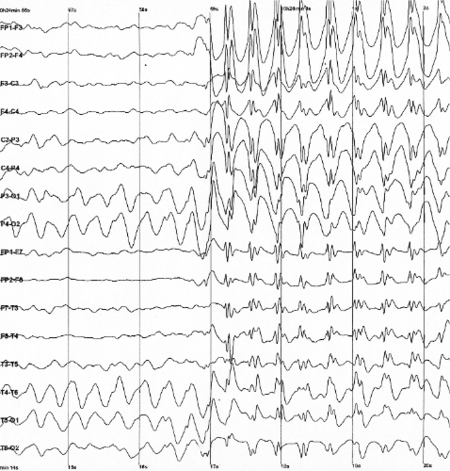
\includegraphics[width=.40\linewidth,height=.30\linewidth]{images/eeg2}}~~~
    %\subfigure[sigma=4]{\label{sigma_4}\includegraphics[width=4cm]{graphs/ex_k3_n500_s4}}~~~
    %\caption{Représentation graphique de l'influence du sigma}
    %\label{sigma}
\end{figure}

\end{frame}

\begin{frame}
\frametitle{L'observation de l'activité cérébrale}
Apprentissage automatique
\begin{itemize}
	\item classification des signaux enregistrés pour reconnaitre l'activité cérébrale mesurée
	\item pallier au manque de précision des signaux
\end{itemize}
~\\
Algorithmes évolutionnistes
\begin{itemize}
	\item recherche de caractéristiques [GPAT03] [SBR03]
	\item optimiser la topologie du classifieur [BSHEB97]
\end{itemize}
\end{frame}

\begin{frame}
\frametitle{Conclusion}
L'utilisation des algorithmes évolutionnistes dans les neurosciences computationnelles :
\begin{itemize}
	\item l'analyse et l'optimisation de modèles biologiques
    \item l'optimisation de modèles \og~boite noire~\fg
    \item l'observation de l'activité cérébrale
\end{itemize}
\end{frame}

\begin{frame}[allowframebreaks]
\frametitle{Bibliographie}
\begin{itemize}
    \item $[$BCM02$]$
    B.~Blankertz, G.~Curio, and K.R. Muller, \emph{{Classifying single trial
      EEG: Towards brain computer interfacing}}, Advances in neural information
      processing systems: proceedings of the 2002 conference, MIT Press, 2002,
      p.~157.

    \item $[$BLV07$]$
    O.~Bai, P.~Lin, S.~Vorbach, J.~Li, S.~Furlani, and M.~Hallett,
      \emph{{Exploration of computational methods for classification of movement
      intention during human voluntary movement from single trial EEG}}, Clinical
      Neurophysiology (2007).

    \item $[$BSHEB97$]$
    R.~Baumgart-Schmitt, WM~Herrmann, R.~Eilers, and F.~Bes, \emph{{On the Use of
      Neural Network Techniques to Analyse Sleep EEG Data First Communication:
      Application of Evolutionary and Genetic Algorithms to Reduce the Feature
      Space and to Develop Classification Rules}}, NEUROPSYCHOBIOLOGY-BASEL-
      \textbf{36} (1997), 194--210.

    \item $[$DMW08$]$
    F.~Dohler, F.~Mormann, B.~Weber, C.E. Elger, and K.~Lehnertz, \emph{{A
      cellular neural network based method for classification of magnetic resonance
      images: Towards an automated detection of hippocampal sclerosis}}, Journal of
      Neuroscience Methods \textbf{170} (2008), no.~2, 324--331.

    \item $[$DBG07$]$
    Druckmann, S. and Banitt, Y. and Gidon, A. and Sch{\\"u}rmann, F. and Markram, H. and Segev, I.,
      \emph{{A novel multiple objective optimization framework for constraining conductance-based neuron models by experimental data}},
      Frontiers in neuroscience \textbf{1} (2007), no.~1, p7.

    \item $[$GPAT03$]$
    D.~Garrett, D.A. Peterson, C.W. Anderson, and M.H. Thaut, \emph{{Comparison of
      linear and nonlinear methods for EEG signal classification}}, IEEE
      Transactions on Neural Systems and Rehabilitative Engineering \textbf{11}
      (2003), no.~2, 141--144.

    \item $[$HGP05$]$
    Humphries, M.D. and Gurney, K. and Prescott, T.J., \emph{{Is there an integrative center in the vertebrate brain-stem?}},
      Adaptive Behavior \textbf{13}, 2005, no.~2, 97.

    \item $[$HO97$]$
    N.~Hansen and A.~Ostermeier, \emph{{Convergence Properties of Evolution
      Strategies with the Derandomized Covariance Matrix Adaptation}},
      Eufit \textbf{97}, 650--654.

    \item $[$HO01$]$
    N.~Hansen and A.~Ostermeier, \emph{{Completely derandomized self-adaptation in evolution
      strategies}}, Evolutionary computation \textbf{9} (2001), no.~2, 159--195.

    \item $[$KPK05$]$
    Keren, N. and Peled, N. and Korngreen, A., \emph{{Constraining compartmental models using multiple voltage recordings and genetic algorithms}},
      Journal of neurophysiology \textbf{94} (2005), no.~6, 3730.

    \item $[$MAR06$]$
    Markram H., \emph{{The blue brain project}},
      Nature Reviews Neuroscience \textbf{7} (2006), no.~2, 153--159.

    \item $[$SBR03$]$
    M.~Schroder, M.~Bogdan, W.~Rosenstiel, T.~Hinterberger, and N.~Birbaumer,
      \emph{{Automated EEG feature selection for brain computer interfaces}},
      Proceedings of the 1st International IEEE EMBS Conference on Neural
      Engineering, 2003, pp.~626--629.

    \item $[$SIK04$]$
    S.~Schneider, C.~Igel, C.~Klaes, H.R. Dinse, and J.C. Wiemer,
      \emph{{Evolutionary adaptation of nonlinear dynamical systems in
      computational neuroscience}}, Genetic Programming and Evolvable Machines
      \textbf{5} (2004), no.~2, 215--227.

    \item $[$WN03$]$
    T.D. Wager and T.E. Nichols, \emph{{Optimization of experimental design in
      fMRI: a general framework using a genetic algorithm}}, Neuroimage \textbf{18}
      (2003), no.~2, 293--309.

    \item $[$WLCH07$]$
    Wang, Y. and Li, S. and Chen, Q. and Hu, W., \emph{{Biology Inspired Robot Behavior Selection Mechanism: Using Genetic Algorithm}},
    LECTURE NOTES IN COMPUTER SCIENCE \textbf{4688}
      (2007), 777.

    \item $[$YF08$]$
    J.Y. Yeh and JC~Fu, \emph{{A hierarchical genetic algorithm for segmentation of
      multi-spectral human-brain MRI}}, Expert Systems with Applications
      \textbf{34} (2008), no.~2, 1285--1295.
\end{itemize}
\end{frame}

\begin{frame}
%\frametitle{Licences}
\begin{center}
    \href{http://creativecommons.org/licenses/by-sa/2.0/fr/}{
\includegraphics[width=.40\linewidth]{images/cc_by_sa}}
    \\[3em]
    \textbf{Illustrations}\\\medskip
    %\begin{tabular}{ l l }
    %Johann "nojhan" Dréo & 
\includegraphics[height=1em]{images/cc_by_sa_small} \\
    %\end{tabular}
    %
\includegraphics[height=1em]{images/cc_by_sa_small}
    \href{http://commons.wikimedia.org/wiki/User:Nojhan}{Johann "nojhan" Dréo} \raisebox{-0.5\height+0.3em}{\href{http://creativecommons.org/licenses/by-sa/2.0/fr/}{
\includegraphics[height=1em]{images/cc_by_sa_small}}}
\end{center}
\end{frame}

\end{document}
